\section{Image Segmentation}
Although the primary deliverable of the project was not to invent a new image segmentation algorithm, the method of image segmentation was an important choice.

It was decided that a depth-sensing camera~\cite{xtion} would be used in order to assist with region extraction. Rather than relying solely on RGB data and difference in colour to extract objects from the video footage, depth data would also be considered. This choice was made, as object-segmentation was desired --- if a white cup was placed on a white table, traditional colour-based segmentation algorithms may struggle to differentiate between the object and the surfact on which the object was sitting.

As majority of image segmentation algorithm implmentations consider only colour information for segmentation; it was not possible to use an off-the-shelf MATLAB module to complete this task. After reviewing publications on segmentation using both depth and RGB data, a few different approaches were trialled.

\subsection{Standard Deviation}
As an intial experiment, I attempted to highlight ``interesting'' sections of the image. This was accomplished by using a sliding window over the RGB image, calculating the standard deviation of the pixels in the window. The resulting image was then thresholded and used on a mask on the orignal image,

This method was quite succesful - the resulting image only contained objects that stood out on the input image.

\begin{figure}[H]
    \centering
    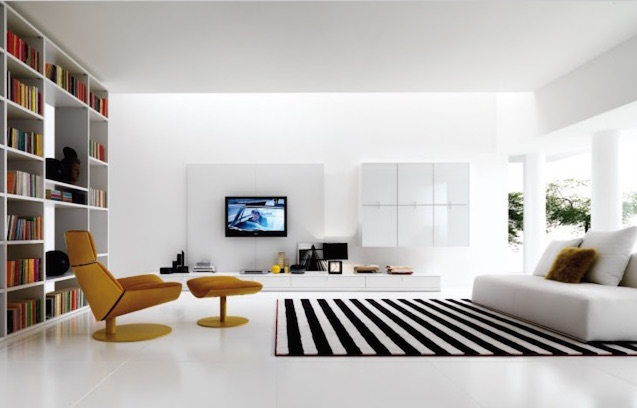
\includegraphics[width=0.6\textwidth]{Segmentation/sd-input.jpg}
    \caption{Input Image}
\end{figure}

\begin{figure}[H]
   \centering
   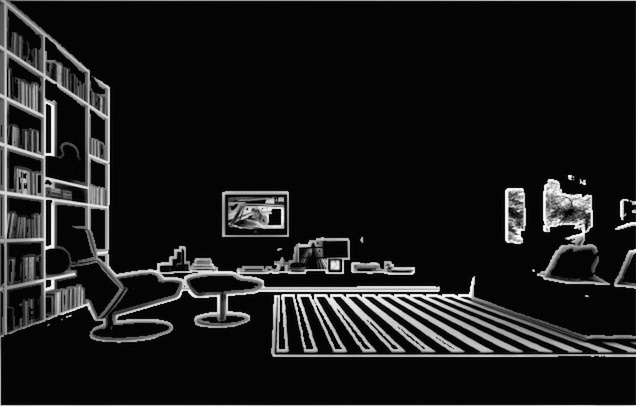
\includegraphics[width=0.6\textwidth]{Segmentation/sd-output.jpg}
   \caption{Standard Deviation Results}

\end{figure}

The main issue with this approach was that Depth Information was not used - cases where objects had little RGB contrast would not be picked out. 

\subsection{K-Means with 4 channels}
One approach was to use a standard K-Means image segmentation algorithm~\cite{kmeans-matlab}, with an additional channel added, representing depth. 
\begin{figure}
    \centering

    \begin{subfigure}[b]{0.5\textwidth}
        \centering
        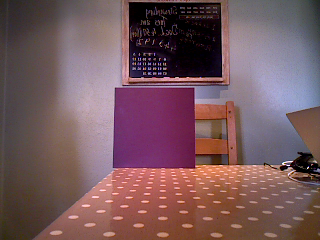
\includegraphics[width=textwidth]{Segmentation/squarergb-10.png}
        \caption{Input RGB image}
    \end{subfigure}

    \hfill

    \begin{subfigure}[b]{0.5\textwidth}
        \centering
        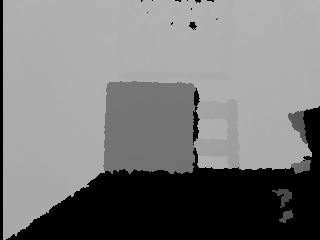
\includegraphics[width=textwidth]{Segmentation/squaredepth-10.png}
        \caption{Input Depth Map}
    \end{subfigure}
\end{figure}

\begin{figure}[H]
\centering
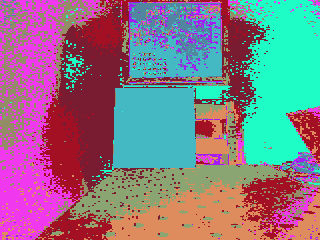
\includegraphics[width=0.4\textwidth]{Segmentation/kmeans-rgb-10seg-im9.png}
\caption{RGB-only K-Means segmentation}
\end{figure}

\begin{figure}[H]
\centering
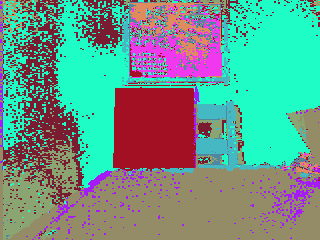
\includegraphics[width=0.4\textwidth]{Segmentation/kmeans-rgb-depth-10seg-im9.png}
\caption{RGBD K-means segmentation}
\end{figure}

This was fairly succesful, however was very vulnerable to noise - only images acquired in environments with perfect lighting provided good segmentation results. 

These results were fairly good - the addition of the depth channel resulted in a smoother segmentation. However, using raw images from the camera for segmentation resulted in a fairly noisy image. Applying a gaussian blur to the image (\diameter = 5, \sigma = 2) removed some of the noise, at the expense of sharpness in the image.

\begin{figure}[H]
\centering
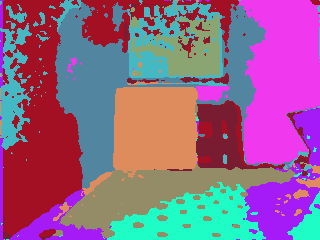
\includegraphics[width=0.4\textwidth]{Segmentation/rgb-depth-kmeans-blurred-10.png}
\caption{Segmentation of blurred RGBD image}
\end{figure}

\subsection{K-Nearest Neighbour}

\subsection{Channel Swapping}
As mentioned, most segmentation algorithms support only RGB data. With this in mind, another approach taken was to remove a colour channel from the RGB image, and swap it with the depth image. This was quite sucessful --- the resulting segmentation was more accurate than either RGB or Depth alone.

\subsection{Graph Cuts}
Attempts were made to use the Graph Cuts algoritm [REF] in order to segment the video and depth data. However, it became apparent that this approach was taking orders of magnitude longer than we could reasonably spend processing each frame; we wanted the system to run as close to real-time as possible.

\section{Feature Extraction}

\subsection{Basis Shapes}

\subsubsection{Zernike Moments}
Zernike Moments ---ref--- are a set of orthogonal moments ---EXPAND---. Due to their orthogonality, it is possible for a computer to compress an image or shape very efficiently using Zernike Moments. 

With this in mind, I attempted to express the extracted shape in terms of Zernike Moments --- the theory being that given the Zernike moments, a human may be able to re-construct the image mentally.

By assigning a harmonic to each Zernike moment, and varying the amplitude of each harmonic according to the moment value, a tone was generated. I then proceeded to pass various shapes into the algorithm, listening to the tone.

Although the tone varied with each shape, it was not possible to identify individual shapes using this system --- it was unclear how a change in the amplitude of a particular harmonic corresponded to changes in shape. 

